\documentclass[10pt,]{article}
\usepackage{lmodern}
\usepackage{setspace}
\setstretch{1.3}
\usepackage{amssymb,amsmath}
\usepackage{ifxetex,ifluatex}
\usepackage{fixltx2e} % provides \textsubscript
\ifnum 0\ifxetex 1\fi\ifluatex 1\fi=0 % if pdftex
  \usepackage[T1]{fontenc}
  \usepackage[utf8]{inputenc}
\else % if luatex or xelatex
  \ifxetex
    \usepackage{mathspec}
    \usepackage{xltxtra,xunicode}
  \else
    \usepackage{fontspec}
  \fi
  \defaultfontfeatures{Mapping=tex-text,Scale=MatchLowercase}
  \newcommand{\euro}{€}
\fi
% use upquote if available, for straight quotes in verbatim environments
\IfFileExists{upquote.sty}{\usepackage{upquote}}{}
% use microtype if available
\IfFileExists{microtype.sty}{%
\usepackage{microtype}
\UseMicrotypeSet[protrusion]{basicmath} % disable protrusion for tt fonts
}{}
\usepackage[margin=1in]{geometry}
\usepackage{longtable,booktabs}
\usepackage{graphicx}
\makeatletter
\def\maxwidth{\ifdim\Gin@nat@width>\linewidth\linewidth\else\Gin@nat@width\fi}
\def\maxheight{\ifdim\Gin@nat@height>\textheight\textheight\else\Gin@nat@height\fi}
\makeatother
% Scale images if necessary, so that they will not overflow the page
% margins by default, and it is still possible to overwrite the defaults
% using explicit options in \includegraphics[width, height, ...]{}
\setkeys{Gin}{width=\maxwidth,height=\maxheight,keepaspectratio}
\ifxetex
  \usepackage[setpagesize=false, % page size defined by xetex
              unicode=false, % unicode breaks when used with xetex
              xetex]{hyperref}
\else
  \usepackage[unicode=true]{hyperref}
\fi
\hypersetup{breaklinks=true,
            bookmarks=true,
            pdfauthor={Marcelo G. Nunes, Julio A. Z. Trecenti},
            pdftitle={Reformas de decisão nas câmaras de direito criminal em São Paulo},
            colorlinks=true,
            citecolor=blue,
            urlcolor=blue,
            linkcolor=magenta,
            pdfborder={0 0 0}}
\urlstyle{same}  % don't use monospace font for urls
\setlength{\parindent}{0pt}
\setlength{\parskip}{6pt plus 2pt minus 1pt}
\setlength{\emergencystretch}{3em}  % prevent overfull lines
\setcounter{secnumdepth}{0}

%%% Use protect on footnotes to avoid problems with footnotes in titles
\let\rmarkdownfootnote\footnote%
\def\footnote{\protect\rmarkdownfootnote}

%%% Change title format to be more compact
\usepackage{titling}

% Create subtitle command for use in maketitle
\newcommand{\subtitle}[1]{
  \posttitle{
    \begin{center}\large#1\end{center}
    }
}

\setlength{\droptitle}{-2em}
  \title{\LARGE Reformas de decisão nas câmaras de direito criminal em São Paulo}
  \pretitle{\vspace{\droptitle}\centering\huge}
  \posttitle{\par}
  \author{Marcelo G. Nunes, Julio A. Z. Trecenti}
  \preauthor{\centering\large\emph}
  \postauthor{\par}
  \predate{\centering\large\emph}
  \postdate{\par}
  \date{2015-07-14}



\begin{document}

\maketitle


\paragraph{Marcelo Guedes Nunes}\label{marcelo-guedes-nunes}

~

Doutor em Direito pela Pontifícia Universidade Católica de São
Paulo.\\Contato eletrônico:
\href{mailto:mnunes@abjur.org.br}{\nolinkurl{mnunes@abjur.org.br}}

\paragraph{Julio Adolfo Zucon
Trecenti}\label{julio-adolfo-zucon-trecenti}

~

Mestrando em Estatística pelo Instituto de Matemática e Estatística da
Universidade de São Paulo.\\Contato eletrônico:
\href{mailto:jtrecenti@abjur.org.br}{\nolinkurl{jtrecenti@abjur.org.br}}

\subsection{Introdução}\label{introducao}

O Direito Criminal é uma área que traz consigo diversas questões
difíceis e importantes da nossa sociedade. Uma destas questões, que
remete ao possível descolamento da teoria do Direito e o que ocorre no
mundo real, trata do cumprimento da pena. Considerando-se o plano ideal
e o princípio de ampla defesa, mas também a conhecida morosidade dos
tribunais, qual é o momento do processo em que deveria ser iniciado o
cumprimento de pena? Será que a taxa de reforma das decisões é tão
pequena a ponto de justificar o início do cumprimento de pena após a
sentença na primeira instância?

Com o objetivo de obter essas taxas, a presente pesquisa utiliza como
base de dados um levantamento de 157.379 decisões em segunda instância,
das quais pouco menos de 60.000 envolvem apelações contra o Ministério
Público, todas proferidas entre 01/01/2014 e 31/12/2014 nas dezesseis
Câmaras de Direito Criminal do Estado de São Paulo, e nas Câmaras
Extraordinárias. Todas as informações foram obtidas através de
ferramentas computacionais a partir de bases de dados disponíveis
publicamente, o que permitiria a reprodutibilidade da pesquisa. Os dados
semiestruturados foram organizados a partir da utilização de técnicas de
mineração de texto. Também foi necessário utilizar procedimentos
estatísticos adequados para lidar com problemas de dados faltantes.

Os resultados ainda preliminares, surpreendentemente, revelam taxas de
reforma que corroboram de forma aproximada com o clássico teorema
desenvolvido em Priest \& Klein (1984) sobre taxas de provimento e viés
de seleção, mesmo tendo os autores criado a teoria para casos cíveis.
Como mostram os autores, as taxas de improvimento de processos, nos
grandes números, seguem uma tendência de se aproximarem de 50\% do total
das decisões. Tal resultado é recorrente em diversas áreas do Direito
como, por exemplo, em processos tributários.

O estudo aponta para taxas de reforma de decisões e exclusão da
punibilidade não muito elevadas, mas que também podem não ser
negligíveis a ponto de justificar a ideia de adiantamento do início do
cumprimento de pena para a decisão em primeira instância. Com o intuito
de complementar e aprofundar a pesquisa, realizamos análises para tipos
específicos de crime, como roubo e tráfico de drogas, comparando as
taxas de reforma em cada subpopulação. Realizamos também a comparação
dos resultados relativamente às câmaras de julgamento e relatores.

Acreditamos que o estudo possa servir como base de informação
quantitativa para auxiliar nas discussões correntes sobre o melhor
momento para dar início ao cumprimento de pena.

\subsection{Motivação}\label{motivacao}

Por conta da ascenção da mídia nas redes sociais, escândalos de
corrupção e o aumento das discussões políticas, o tema da impunidade
aparece de forma mais explícita. Uma das principais questões que surgem
quando o tema é impunidade e que gerou as ideias iniciais desse artigo
é: quando um réu condenado deve começar a cumprir pena? A justiça deve
esperar o encerramento definitivo do processo, com o chamado trânsito em
julgado, ou pode iniciar o cumprimento já a partir de uma decisão
terminativa, como a sentença ou o acórdão de segundo grau?

A resposta intuitiva seria aguardar a condenação definitiva, para evitar
que um réu comece a cumprir pena e depois acabe sendo absolvido por um
tribunal superior. Essa é a atual opção do legislador, que, no entanto,
não está imune a problemas decorrentes da demora no processo. A longa
espera pelo trânsito em julgado cria uma sensação de impunidade nas
vítimas, que, não desprovidas de razão, assistem passivas aos
desdobramentos da burocracia processual como uma chancela à impunidade.
Essa sensação se agrava quando os acusados conseguem extinguir os
processos pela prescrição, escapando da pena não por terem provado
inocência, mas pela demora do judiciário em condená-los. Além disso, a
possibilidade de ganhar tempo incentiva uma profusão de recursos e
congestiona os tribunais.

Como reação surgiram as propostas de aceleração dos processos, no
sentido de atribuir eficácia imediata para a sentença de primeira
instância (nos casos de crimes graves em concreto) ou, ainda, de
antecipar o trânsito em julgado para a segunda instância, efetivando a
condenação ainda que haja pendência do julgamento de recursos especial e
extraordinário. As propostas, por sua vez, geraram críticas. Os críticos
da aceleração dos processos argumentam que a presunção de inocência deve
ser respeitada para evitar a injustiça de prender quem não pode ainda se
defender. De outro lado, os defensores das reformas entendem que a ação
do estado deve ser acelerada para evitar a injustiça de não prender quem
cometeu crime.

Se limitarmos a discussão ao plano principiológico, como ela é
tradicionalmente enfrentada pela classe jurídica, fica difícil avançar.
Qual princípio é mais importante: a presunção de inocência ou a
efetividade do processo? Formulada nesses termos, a pergunta não tem uma
reposta aceitável porque nós precisamos das duas coisas: de um processo
que garanta a presunção de inocência e que seja\\ao mesmo tempo efetivo.
É como perguntar se uma pessoa prefere água potável ou ar. Na prática,
queremos os dois: um volume de água que não seja nem tão grande ao ponto
de me matar afogado, nem tão escasso ao ponto de me matar de sede. Isso
nos leva a essência do trabalho da jurimetria, que é quantificar os
efeitos dessas propostas para auxiliar na formulação de políticas
públicas. Portanto, acredito que a questão da aceleração dos processos
deve se preocupar menos com peso abstrato dos princípios e mais com a
estimação da quantidade de pessoas potencialmente afetadas por cada
proposta.

Sobre prisão provisória, XXX (falar do soudapaz)\ldots{}

\subsection{Objetivos}\label{objetivos}

Nossa pesquisa é bastante direta e preliminar. Temos como objetivos

\begin{itemize}
\itemsep1pt\parskip0pt\parsep0pt
\item
  Estimar a taxa de reforma de decisões nas câmaras de direito criminal
  em São Paulo.
\item
  Desagregar essa taxa de acordo com outras informações processuais.
\item
  Discutir os resultados e propor novas análises.
\end{itemize}

\subsection{Dados}\label{dados}

Os dados foram obtidos via \emph{web scraping}, ou raspagem de dados a
partir das informações disponíveis no Tribunal de Justiça de São Paulo.
A pesquisa foi realizada utilizando-se um pacote construído com o
software estatístico R. O código fonte do estudo está disponível e a
pesquisa poderia ser replicada com diferentes configurações\footnote{Código
  disponível em
  \href{https://github.com/jtrecenti/tjspCrim}{\url{https://github.com/jtrecenti/tjspCrim}}.}.

A extração e estruturação de dados passou por três fases principais: a
listagem de acórdãos, o download das informações dos processos e a
manipulação dos dados e text mining para obtenção da base de dados
finais.

\subsubsection{Listagem de acórdãos}\label{listagem-de-acordaos}

A listagem dos processos foi feita a partir da busca de jurisprudência
disponível na ferramenta e-SAJ do TJSP\footnote{Acesse
  \href{https://esaj.tjsp.jus.br/cjsg/resultadoCompleta.do}{\url{https://esaj.tjsp.jus.br/cjsg/resultadoCompleta.do}}
  para visualizar a página utilizada na pesquisa.}. Fizemos a busca da
forma menos restritiva possível, limitando apenas aos 146 órgãos
julgadores definidos na seção ``Direito Criminal'' na página de pesquisa
e limitando as datas de julgamento entre 01/01/2014 até 31/12/2014.

A consulta retornou um total de 157.379 acórdãos. Pelo que vimos em
outras pesquisas, esse número pode mudar um pouco caso a pesquisa seja
realizada em momentos diferentes, mesmo que o período da pesquisa esteja
no passado. Na nossa consulta mais recente, realizada em 13/07/2015, a
consulta retornou 157.412 resultados.

A partir da utilização do robô construído, foi possível acessar todas as
páginas resultantes da consulta e obter as seguintes informações, ainda
em formato semi-estruturado (HTML) ou não estruturado (textos livres).
As informações incluem número do processo, código do acórdão (interno do
sistema SAJ), classe / assunto, texto sem formatação, nome do relator,
comarca de origem, órgão julgador, data do julgamento, data do registro
e ementa.

A informação mais relevante nessa pesquisa é o número do processo. O
número foi utilizado para acessar os processos usando outra ferramenta
de pesquisa do e-SAJ.

\subsubsection{Download de informações dos
processos}\label{download-de-informacoes-dos-processos}

A segunda etapa para obtenção dos dados foi obter informações extras a
partir da consulta de processos do segundo grau no e-SAJ\footnote{Acesse
  \href{https://esaj.tjsp.jus.br/cpo/sg/open.do}{\url{https://esaj.tjsp.jus.br/cpo/sg/open.do}}
  para visualizar a página utilizada na pesquisa.}. Para atender os
objetivos da pesquisa, no entanto, fizemos um filtro inicial nos dados.
Observe as classes processuais contidas na Tabela 1. Como nosso
interesse é somente nas apelações, realizamos um primeiro filtro na base
original, buscando apenas decisões com essa classe processual,
resultando em 68.238 decisões.

\begin{longtable}[c]{@{}lrc@{}}
\caption{Tabela de frequências das classes processuais.}\tabularnewline
\toprule
classe & n & \%\tabularnewline
\midrule
\endfirsthead
\toprule
classe & n & \%\tabularnewline
\midrule
\endhead
Apelação & 68238 & 43.4\%\tabularnewline
Habeas Corpus & 49061 & 31.2\%\tabularnewline
Agravo de Execução Penal & 24877 & 15.8\%\tabularnewline
Embargos de Declaração & 4825 & 3.1\%\tabularnewline
Revisão Criminal & 3919 & 2.5\%\tabularnewline
Recurso em Sentido Estrito & 3038 & 1.9\%\tabularnewline
Agravo Regimental & 1342 & 0.9\%\tabularnewline
Outros & 1147 & 0.7\%\tabularnewline
Mandado de Segurança & 932 & 0.6\%\tabularnewline
Total & 157379 & 100.0\%\tabularnewline
\bottomrule
\end{longtable}

A partir da lista de processos, utilizamos a página do e-SAJ para
consulta de processos de segundo grau. Na base de dados filtrada, temos
somente 68.044 números de processos únicos (os números duplicados
correspondem a processos com mais de uma apelação, e.g., apelação do
ministério público e do réu).

Utilizando ferramentas semelhantes à da subseção anterior para raspagem
dos dados, conseguimos obter informações do texto da decisão, partes e
andamentos dos processos. Essas informações foram então incorporadas à
base de dados original filtrada.

\subsubsection{Manipulação e text
mining}\label{manipulacao-e-text-mining}

O último passo para a obtenção da base de dados final é também o mais
trabalhoso. A consolidação envolve a manipulação e limpeza dos dados,
além da extração de informações dos textos.

Nessa pesquisa, consideramos no escopo somente apelações realizadas
contra o Ministério Público. Assim, incluímos na base somente processos
em que o réu apelava para pedir cancelamento, redução de pena, etc. Após
esse filtro ficamos com uma base contendo 57.625 processos.

Para obter as decisões dos processos, fizemos um \emph{text mining} dos
textos das decisoes, extraindo os resultados a partir de regras lógicas
e expressões regulares. Os resultados não são totalmente a prova de
erros, mas é provavel que as classificações estejam próximas da
realidade.

Não foi possível classificar a decisão de 618 casos e, por conta disso,
as análises precisam utilizar técnicas que lidam de forma adequada com
dados faltantes. Para isso, utilizamos imputação de dados utilizando o
modelo Amelia II (Gary King et. al., 2011).

\subsubsection{Base de dados final}\label{base-de-dados-final}

A base de dados final contém 57.625 linhas e 7 colunas, com as seguintes
variáveis:

\begin{itemize}
\itemsep1pt\parskip0pt\parsep0pt
\item
  Número do processo: número CNJ identificador do processo.
\item
  Relator: nome do relator.
\item
  Comarca: nome da comarca de origem do processo.
\item
  Órgão Julgador: câmara de direito criminal.
\item
  Data de julgamento: data do julgamento do processo.
\item
  Assunto: assunto do processo, na maioria das vezes classificado a
  partir da resolução 65 do CNJ.
\item
  Decisão: decisão do processo.
\end{itemize}

\subsection{Resultados}\label{resultados}

A Tabela XXX mostra o a distribuição das decisões dos processos. É
interessante notar que a taxa de decisões desfavoráveis é de
aproximadamente 50\%, o que vai de encontro com o resultado apresentado
por Priest \& Klein (1984).

\begin{longtable}[c]{@{}lrc@{}}
\caption{Tabela de frequências dos resultados dos
processos.}\tabularnewline
\toprule
decisao & n & \%\tabularnewline
\midrule
\endfirsthead
\toprule
decisao & n & \%\tabularnewline
\midrule
\endhead
negaram & 31059 & 53.9\%\tabularnewline
parcialmente & 17877 & 31.0\%\tabularnewline
provido & 8342 & 14.5\%\tabularnewline
outros & 347 & 0.6\%\tabularnewline
Total & 57625 & 100.0\%\tabularnewline
\bottomrule
\end{longtable}

O modelo apresentado por Priest e Klein utiliza é baseado em um viés de
seleção que considera a qualidade do recurso e as expectativas das
partes em relação a esse recurso. Vamos ilustrar isso no caso cível. Por
um lado, se ambas as partes acreditam que o autor tem razão, o réu tende
a oferecer um acordo. Por outro lado, se ambas as partes acreditam que o
réu tem razão, então o autor não chega a litigar. O litígio ocorre
quando existe uma diferença nas expectativas das partes em relação ao
processo, ou seja, quando ambos acreditam que vão ganhar. Isso faz com
que somente casos com maior incerteza de resultado cheguem a julgamento,
de forma que, sob certas suposições, a proporção final de resultados
favoráveis tenda ao valor de 50\%.

No caso criminal, no entanto, o acordo entre as partes não existe. Isso
seria suficiente para invalidar o modelo de Priest e Klein. O único
estudo já feito sobre viés de seleção em casos criminais é encontrado em
Klerman (2000), e ele só foi possível pois a pesquisa é baseada em
processos do século XIII, ainda na idade média, que segundo o autor
incluiam a possibilidade de acordo.

Ainda assim, encontramos na nossa pesquisa um valor muito próximo de
50\%. Esse é um resultado bastante intrigante, que poderia ser fruto do
acaso, mas poderia também ser a aplicação de um modelo de seleção ainda
desconhecido na academia. Neste artigo, não almejamos construir tal
modelo, e o que fizemos foi simplesmente investigar o que ocorre com os
resultados em algumas subpopulações.

\paragraph{Comarca de origem}\label{comarca-de-origem}

A Tabela XXX mostra a distribuição dos resultados dos processos em
relação às quinze comarcas com maior volume processual. Podemos notar
que o padrão muda de forma significativa em cada comarca. Piracicaba,
Santo André e Campinas apresentam taxas de apelações negadas acima de
60\%, enquanto Mogi das Cruzes e Sumaré apresentam taxas menores do que
45\%. Num contexto de viés de seleção, estas diferenças podem ser
significativas e podem indicar que o perfil dos processos e/ou decisões
em primeira instância nessas comarcas pode ser diferente.

\begin{longtable}[c]{@{}rrrrrr@{}}
\caption{Tabela de frequências dos resultados dos processos segundo
comarca.}\tabularnewline
\toprule
Comarca & negaram & outros & parcialmente & provido &
total\tabularnewline
\midrule
\endfirsthead
\toprule
Comarca & negaram & outros & parcialmente & provido &
total\tabularnewline
\midrule
\endhead
São Paulo & 7049 (57.5\%) & 54 (0.4\%) & 3939 (32.1\%) & 1212 (9.9\%) &
12254 (100\%)\tabularnewline
Campinas & 848 (60.7\%) & 8 (0.6\%) & 380 (27.2\%) & 162 (11.6\%) & 1398
(100\%)\tabularnewline
Guarulhos & 662 (53.4\%) & 12 (1.0\%) & 443 (35.7\%) & 123 (9.9\%) &
1240 (100\%)\tabularnewline
São Bernardo do Campo & 577 (54.5\%) & 6 (0.6\%) & 364 (34.4\%) & 111
(10.5\%) & 1058 (100\%)\tabularnewline
São José dos Campos & 539 (53.5\%) & 7 (0.7\%) & 315 (31.3\%) & 146
(14.5\%) & 1007 (100\%)\tabularnewline
Ribeirão Preto & 579 (59.1\%) & 5 (0.5\%) & 246 (25.1\%) & 150 (15.3\%)
& 980 (100\%)\tabularnewline
Piracicaba & 626 (64.0\%) & 4 (0.4\%) & 227 (23.2\%) & 121 (12.4\%) &
978 (100\%)\tabularnewline
São José do Rio Preto & 490 (58.2\%) & 3 (0.4\%) & 211 (25.1\%) & 138
(16.4\%) & 842 (100\%)\tabularnewline
Santos & 495 (58.9\%) & 6 (0.7\%) & 233 (27.7\%) & 107 (12.7\%) & 841
(100\%)\tabularnewline
Sorocaba & 399 (54.3\%) & 4 (0.5\%) & 262 (35.6\%) & 70 (9.5\%) & 735
(100\%)\tabularnewline
Sumaré & 309 (44.9\%) & 3 (0.4\%) & 260 (37.8\%) & 116 (16.9\%) & 688
(100\%)\tabularnewline
Santo André & 375 (61.1\%) & 2 (0.3\%) & 181 (29.5\%) & 56 (9.1\%) & 614
(100\%)\tabularnewline
Franca & 341 (57.0\%) & 3 (0.5\%) & 180 (30.1\%) & 74 (12.4\%) & 598
(100\%)\tabularnewline
Mogi das Cruzes & 255 (42.8\%) & 4 (0.7\%) & 259 (43.5\%) & 78 (13.1\%)
& 596 (100\%)\tabularnewline
total & 31059 (53.9\%) & 347 (0.727\%) & 17877 (31\%) & 8342 (14.5\%) &
57625 (100\%)\tabularnewline
\bottomrule
\end{longtable}

\subsubsection{Assunto}\label{assunto}

Em relação ao assunto, é de se esperar que este tenha um efeito
relevante no resultado das apelações, principalmente por conta da
gravidade do crime e da dificuldade na elaboração de provas. Por outro
lado, por conta da existência do viés de seleção, essas diferenças podem
parecer menores do que realmente são.

A Tabela XXX mostra a distribuição dos resultados dos processos em
relação aos vinte assuntos com maior volume processual. Podemos
verificar uma grande variabilidade nos resultados dos processos,
considerando-se o viés de seleção inerente. Os assuntos com maiores
taxas de recursos negados são homicídio qualificado, latrocínio, roubo e
estupro de vulnerável, justamente os tipos de crimes considerados mais
graves. Os três assuntos com menores taxas de recursos negados são os
crimes de trânsito e violação de direito autoral e outros assuntos, que
agrupa todos os assuntos trinta ou menos processos.

\begin{longtable}[c]{@{}rrrrrr@{}}
\caption{Tabela de frequências dos resultados dos processos segundo
assunto.}\tabularnewline
\toprule
Assunto & negaram & outros & parcialmente & provido &
total\tabularnewline
\midrule
\endfirsthead
\toprule
Assunto & negaram & outros & parcialmente & provido &
total\tabularnewline
\midrule
\endhead
Tráfico de Drogas e Condutas Afins & 8640 (58.3\%) & 50 (0.3\%) & 5096
(34.4\%) & 1041 (7.0\%) & 14827 (100\%)\tabularnewline
Roubo Majorado & 5431 (57.9\%) & 29 (0.3\%) & 3454 (36.8\%) & 462
(4.9\%) & 9376 (100\%)\tabularnewline
Furto Qualificado & 2814 (45.6\%) & 25 (0.4\%) & 2112 (34.2\%) & 1220
(19.8\%) & 6171 (100\%)\tabularnewline
Furto & 1580 (46.4\%) & 23 (0.7\%) & 1003 (29.4\%) & 800 (23.5\%) & 3406
(100\%)\tabularnewline
Crimes do Sistema Nacional de Armas & 1462 (59.3\%) & 6 (0.2\%) & 645
(26.2\%) & 351 (14.2\%) & 2464 (100\%)\tabularnewline
Roubo & 1487 (61.9\%) & 11 (0.5\%) & 791 (32.9\%) & 114 (4.7\%) & 2403
(100\%)\tabularnewline
Receptação & 1100 (50.2\%) & 7 (0.3\%) & 671 (30.6\%) & 414 (18.9\%) &
2192 (100\%)\tabularnewline
Crimes de Trânsito & 724 (36.4\%) & 24 (1.2\%) & 655 (32.9\%) & 586
(29.5\%) & 1989 (100\%)\tabularnewline
Decorrente de Violência Doméstica & 1144 (58.0\%) & 18 (0.9\%) & 457
(23.2\%) & 355 (18.0\%) & 1974 (100\%)\tabularnewline
Estelionato & 685 (46.0\%) & 9 (0.6\%) & 375 (25.2\%) & 420 (28.2\%) &
1489 (100\%)\tabularnewline
Homicídio Qualificado & 876 (66.9\%) & 34 (2.6\%) & 319 (24.4\%) & 81
(6.2\%) & 1310 (100\%)\tabularnewline
Ameaça & 640 (53.9\%) & 6 (0.5\%) & 304 (25.6\%) & 238 (20.0\%) & 1188
(100\%)\tabularnewline
Violação de direito autoral & 309 (40.1\%) & 6 (0.8\%) & 95 (12.3\%) &
361 (46.8\%) & 771 (100\%)\tabularnewline
Uso de documento falso & 436 (59.2\%) & 5 (0.7\%) & 173 (23.5\%) & 123
(16.7\%) & 737 (100\%)\tabularnewline
Outros assuntos & 268 (41.5\%) & 14 (2.2\%) & 140 (21.7\%) & 224
(34.7\%) & 646 (100\%)\tabularnewline
Apropriação indébita & 316 (53.4\%) & 4 (0.7\%) & 135 (22.8\%) & 137
(23.1\%) & 592 (100\%)\tabularnewline
Estupro de vulnerável & 336 (60.0\%) & 5 (0.9\%) & 163 (29.1\%) & 56
(10.0\%) & 560 (100\%)\tabularnewline
Latrocínio & 254 (63.5\%) & 2 (0.5\%) & 121 (30.2\%) & 23 (5.8\%) & 400
(100\%)\tabularnewline
Estupro & 200 (57.8\%) & 2 (0.6\%) & 104 (30.1\%) & 40 (11.6\%) & 346
(100\%)\tabularnewline
total & 31059 (53.9\%) & 347 (0.617\%) & 17877 (31\%) & 8342 (14.5\%) &
57625 (100\%)\tabularnewline
\bottomrule
\end{longtable}

\subsubsection{Órgão julgador}\label{orgao-julgador}

Em relação ao órgão julgador espera-se, a priori, que o órgão não
influencie na distribuição das decisões dos processos, pois os processos
dentro de cada câmara podem ser considerados homogêneos. Essa explicação
só seria válida, no entanto, em relação às câmaras ordinárias, pois as
câmaras extraordinárias julgam, em teoria, processos com características
distintas.

A Tabela XXX mostra a distribuição dos resultados dos processos em
relação ao tipo de órgão julgador. Na comparação, é possível notar que
as câmaras extraordinárias apresentam uma ligeira superioridade em
relação à proporção de recursos negados, no entanto, essa diferença não
chega perto das diferenças encontradas entre algumas câmaras ordinárias.

\begin{longtable}[c]{@{}rrrrrr@{}}
\caption{Tabela de frequências dos resultados dos processos segundo tipo
de órgão julgador.}\tabularnewline
\toprule
Tipo & negaram & outros & parcialmente & provido & total\tabularnewline
\midrule
\endfirsthead
\toprule
Tipo & negaram & outros & parcialmente & provido & total\tabularnewline
\midrule
\endhead
Ordinária & 23568 (53.0\%) & 294 (0.7\%) & 14745 (33.2\%) & 5860
(13.2\%) & 44467 (100\%)\tabularnewline
Extraordinária & 7491 (56.9\%) & 53 (0.4\%) & 3132 (23.8\%) & 2482
(18.9\%) & 13158 (100\%)\tabularnewline
total & 31059 (53.9\%) & 347 (0.602\%) & 17877 (31\%) & 8342 (14.5\%) &
57625 (100\%)\tabularnewline
\bottomrule
\end{longtable}

Os resultados que seguem são surpreendentes. A Tabela XXX mostra a
distribuição dos resultados dos processos em relação aos órgãos
julgadores. Aqui, encontramos discrepâncias enormes, onde podemos
encontrar câmaras com mais de 75\% de recursos negados (quarta e sexta)
e câmaras com menos de 30\% de recursos negados (primeira, segunda e
décima segunda). Este resultado poderia ser explicado por duas
hipóteses: i) os processos não são distribuídos aleatoriamente nas
câmaras, e é feita uma triagem que envolve a ``qualidade'' do recurso;
ou ii) os magistrados de cada câmara comportam-se de maneiras muito
diferentes, mesmo para processos considerados homogêneos.

\begin{longtable}[c]{@{}rrrrrr@{}}
\caption{Tabela de frequências dos resultados dos processos segundo
órgao julgador.}\tabularnewline
\toprule
Órgão julgador & negaram & outros & parcialmente & provido &
total\tabularnewline
\midrule
\endfirsthead
\toprule
Órgão julgador & negaram & outros & parcialmente & provido &
total\tabularnewline
\midrule
\endhead
4ª Câmara de Direito Criminal & 3084 (81.1\%) & 26 (0.7\%) & 501
(13.2\%) & 192 (5.0\%) & 3803 (100\%)\tabularnewline
3ª Câmara de Direito Criminal & 2294 (65.0\%) & 26 (0.7\%) & 836
(23.7\%) & 375 (10.6\%) & 3531 (100\%)\tabularnewline
14ª Câmara de Direito Criminal & 1796 (52.1\%) & 24 (0.7\%) & 1133
(32.9\%) & 491 (14.3\%) & 3444 (100\%)\tabularnewline
3ª Câmara Criminal Extraordinária & 2418 (71.3\%) & 11 (0.3\%) & 461
(13.6\%) & 499 (14.7\%) & 3389 (100\%)\tabularnewline
4ª Câmara Criminal Extraordinária & 1580 (46.7\%) & 8 (0.2\%) & 1069
(31.6\%) & 728 (21.5\%) & 3385 (100\%)\tabularnewline
9ª Câmara de Direito Criminal & 2211 (68.4\%) & 13 (0.4\%) & 791
(24.5\%) & 219 (6.8\%) & 3234 (100\%)\tabularnewline
1ª Câmara Criminal Extraordinária & 1644 (51.2\%) & 19 (0.6\%) & 868
(27.0\%) & 678 (21.1\%) & 3209 (100\%)\tabularnewline
10ª Câmara de Direito Criminal & 1519 (47.8\%) & 25 (0.8\%) & 1296
(40.8\%) & 335 (10.6\%) & 3175 (100\%)\tabularnewline
2ª Câmara Criminal Extraordinária & 1849 (58.2\%) & 15 (0.5\%) & 734
(23.1\%) & 577 (18.2\%) & 3175 (100\%)\tabularnewline
7ª Câmara de Direito Criminal & 1825 (58.1\%) & 16 (0.5\%) & 891
(28.4\%) & 407 (13.0\%) & 3139 (100\%)\tabularnewline
8ª Câmara de Direito Criminal & 1663 (55.4\%) & 24 (0.8\%) & 736
(24.5\%) & 579 (19.3\%) & 3002 (100\%)\tabularnewline
16ª Câmara de Direito Criminal & 1002 (36.1\%) & 19 (0.7\%) & 1286
(46.4\%) & 467 (16.8\%) & 2774 (100\%)\tabularnewline
11ª Câmara de Direito Criminal & 1282 (46.4\%) & 16 (0.6\%) & 1121
(40.6\%) & 343 (12.4\%) & 2762 (100\%)\tabularnewline
12ª Câmara de Direito Criminal & 412 (15.9\%) & 37 (1.4\%) & 1344
(51.9\%) & 797 (30.8\%) & 2590 (100\%)\tabularnewline
6ª Câmara de Direito Criminal & 2007 (78.8\%) & 25 (1.0\%) & 352
(13.8\%) & 163 (6.4\%) & 2547 (100\%)\tabularnewline
13ª Câmara de Direito Criminal & 1310 (53.3\%) & 15 (0.6\%) & 932
(37.9\%) & 202 (8.2\%) & 2459 (100\%)\tabularnewline
2ª Câmara de Direito Criminal & 542 (23.5\%) & 5 (0.2\%) & 1261 (54.7\%)
& 498 (21.6\%) & 2306 (100\%)\tabularnewline
1ª Câmara de Direito Criminal & 597 (26.9\%) & 9 (0.4\%) & 1198 (54.0\%)
& 414 (18.7\%) & 2218 (100\%)\tabularnewline
5ª Câmara de Direito Criminal & 1260 (71.3\%) & 8 (0.5\%) & 375 (21.2\%)
& 125 (7.1\%) & 1768 (100\%)\tabularnewline
total & 31059 (53.9\%) & 347 (0.602\%) & 17877 (31\%) & 8342 (14.5\%) &
57625 (100\%)\tabularnewline
\bottomrule
\end{longtable}

Uma alternativa para verificar se existe uma diferença nos tipos
processuais dentro de cada câmara é estudar a distribuição dos assuntos
dentro das câmaras. Essa explicação não seria definitiva, afinal pode
ser que sejam separados processos de mesmos assuntos mas com qualidades
diferentes, mas é a verificação que os dados nos permitem realizar.

A Tabela XXX mostra a distribuição de assuntos em cada câmara. Como
temos muitos assuntos, foi necessário agrupar os assuntos com menor
volume em uma categoria. Em relação aos assuntos tráfico de drogas e
condutas afins, furto, furto qualificado e roubo majorado, podemos
identificar algumas diferenças nas distribuições, mas nada que
justifique a grande discrepância observada nos resultados.

\begin{longtable}[c]{@{}ccc@{}}
\caption{Tabela de frequências dos assuntos dos processos segundo órgao
julgador. (continued below)}\tabularnewline
\toprule
\begin{minipage}[b]{0.39\columnwidth}\centering\strut
variavel
\strut\end{minipage} &
\begin{minipage}[b]{0.16\columnwidth}\centering\strut
Furto
\strut\end{minipage} &
\begin{minipage}[b]{0.24\columnwidth}\centering\strut
Furto Qualificado
\strut\end{minipage}\tabularnewline
\midrule
\endfirsthead
\toprule
\begin{minipage}[b]{0.39\columnwidth}\centering\strut
variavel
\strut\end{minipage} &
\begin{minipage}[b]{0.16\columnwidth}\centering\strut
Furto
\strut\end{minipage} &
\begin{minipage}[b]{0.24\columnwidth}\centering\strut
Furto Qualificado
\strut\end{minipage}\tabularnewline
\midrule
\endhead
\begin{minipage}[t]{0.39\columnwidth}\centering\strut
4ª Câmara de Direito Criminal
\strut\end{minipage} &
\begin{minipage}[t]{0.16\columnwidth}\centering\strut
242 (6.4\%)
\strut\end{minipage} &
\begin{minipage}[t]{0.24\columnwidth}\centering\strut
419 (11.0\%)
\strut\end{minipage}\tabularnewline
\begin{minipage}[t]{0.39\columnwidth}\centering\strut
3ª Câmara de Direito Criminal
\strut\end{minipage} &
\begin{minipage}[t]{0.16\columnwidth}\centering\strut
233 (6.6\%)
\strut\end{minipage} &
\begin{minipage}[t]{0.24\columnwidth}\centering\strut
431 (12.2\%)
\strut\end{minipage}\tabularnewline
\begin{minipage}[t]{0.39\columnwidth}\centering\strut
14ª Câmara de Direito Criminal
\strut\end{minipage} &
\begin{minipage}[t]{0.16\columnwidth}\centering\strut
246 (7.1\%)
\strut\end{minipage} &
\begin{minipage}[t]{0.24\columnwidth}\centering\strut
399 (11.6\%)
\strut\end{minipage}\tabularnewline
\begin{minipage}[t]{0.39\columnwidth}\centering\strut
3ª Câmara Criminal Extraordinária
\strut\end{minipage} &
\begin{minipage}[t]{0.16\columnwidth}\centering\strut
230 (6.8\%)
\strut\end{minipage} &
\begin{minipage}[t]{0.24\columnwidth}\centering\strut
397 (11.7\%)
\strut\end{minipage}\tabularnewline
\begin{minipage}[t]{0.39\columnwidth}\centering\strut
4ª Câmara Criminal Extraordinária
\strut\end{minipage} &
\begin{minipage}[t]{0.16\columnwidth}\centering\strut
201 (5.9\%)
\strut\end{minipage} &
\begin{minipage}[t]{0.24\columnwidth}\centering\strut
403 (11.9\%)
\strut\end{minipage}\tabularnewline
\begin{minipage}[t]{0.39\columnwidth}\centering\strut
9ª Câmara de Direito Criminal
\strut\end{minipage} &
\begin{minipage}[t]{0.16\columnwidth}\centering\strut
174 (5.4\%)
\strut\end{minipage} &
\begin{minipage}[t]{0.24\columnwidth}\centering\strut
298 (9.2\%)
\strut\end{minipage}\tabularnewline
\begin{minipage}[t]{0.39\columnwidth}\centering\strut
1ª Câmara Criminal Extraordinária
\strut\end{minipage} &
\begin{minipage}[t]{0.16\columnwidth}\centering\strut
193 (6.0\%)
\strut\end{minipage} &
\begin{minipage}[t]{0.24\columnwidth}\centering\strut
402 (12.5\%)
\strut\end{minipage}\tabularnewline
\begin{minipage}[t]{0.39\columnwidth}\centering\strut
10ª Câmara de Direito Criminal
\strut\end{minipage} &
\begin{minipage}[t]{0.16\columnwidth}\centering\strut
184 (5.8\%)
\strut\end{minipage} &
\begin{minipage}[t]{0.24\columnwidth}\centering\strut
326 (10.3\%)
\strut\end{minipage}\tabularnewline
\begin{minipage}[t]{0.39\columnwidth}\centering\strut
2ª Câmara Criminal Extraordinária
\strut\end{minipage} &
\begin{minipage}[t]{0.16\columnwidth}\centering\strut
196 (6.2\%)
\strut\end{minipage} &
\begin{minipage}[t]{0.24\columnwidth}\centering\strut
410 (12.9\%)
\strut\end{minipage}\tabularnewline
\begin{minipage}[t]{0.39\columnwidth}\centering\strut
7ª Câmara de Direito Criminal
\strut\end{minipage} &
\begin{minipage}[t]{0.16\columnwidth}\centering\strut
188 (6.0\%)
\strut\end{minipage} &
\begin{minipage}[t]{0.24\columnwidth}\centering\strut
330 (10.5\%)
\strut\end{minipage}\tabularnewline
\begin{minipage}[t]{0.39\columnwidth}\centering\strut
8ª Câmara de Direito Criminal
\strut\end{minipage} &
\begin{minipage}[t]{0.16\columnwidth}\centering\strut
131 (4.4\%)
\strut\end{minipage} &
\begin{minipage}[t]{0.24\columnwidth}\centering\strut
258 (8.6\%)
\strut\end{minipage}\tabularnewline
\begin{minipage}[t]{0.39\columnwidth}\centering\strut
16ª Câmara de Direito Criminal
\strut\end{minipage} &
\begin{minipage}[t]{0.16\columnwidth}\centering\strut
151 (5.4\%)
\strut\end{minipage} &
\begin{minipage}[t]{0.24\columnwidth}\centering\strut
298 (10.7\%)
\strut\end{minipage}\tabularnewline
\begin{minipage}[t]{0.39\columnwidth}\centering\strut
11ª Câmara de Direito Criminal
\strut\end{minipage} &
\begin{minipage}[t]{0.16\columnwidth}\centering\strut
181 (6.6\%)
\strut\end{minipage} &
\begin{minipage}[t]{0.24\columnwidth}\centering\strut
293 (10.6\%)
\strut\end{minipage}\tabularnewline
\begin{minipage}[t]{0.39\columnwidth}\centering\strut
12ª Câmara de Direito Criminal
\strut\end{minipage} &
\begin{minipage}[t]{0.16\columnwidth}\centering\strut
171 (6.6\%)
\strut\end{minipage} &
\begin{minipage}[t]{0.24\columnwidth}\centering\strut
253 (9.8\%)
\strut\end{minipage}\tabularnewline
\begin{minipage}[t]{0.39\columnwidth}\centering\strut
6ª Câmara de Direito Criminal
\strut\end{minipage} &
\begin{minipage}[t]{0.16\columnwidth}\centering\strut
167 (6.6\%)
\strut\end{minipage} &
\begin{minipage}[t]{0.24\columnwidth}\centering\strut
264 (10.4\%)
\strut\end{minipage}\tabularnewline
\begin{minipage}[t]{0.39\columnwidth}\centering\strut
13ª Câmara de Direito Criminal
\strut\end{minipage} &
\begin{minipage}[t]{0.16\columnwidth}\centering\strut
102 (4.1\%)
\strut\end{minipage} &
\begin{minipage}[t]{0.24\columnwidth}\centering\strut
235 (9.6\%)
\strut\end{minipage}\tabularnewline
\begin{minipage}[t]{0.39\columnwidth}\centering\strut
2ª Câmara de Direito Criminal
\strut\end{minipage} &
\begin{minipage}[t]{0.16\columnwidth}\centering\strut
136 (5.9\%)
\strut\end{minipage} &
\begin{minipage}[t]{0.24\columnwidth}\centering\strut
239 (10.4\%)
\strut\end{minipage}\tabularnewline
\begin{minipage}[t]{0.39\columnwidth}\centering\strut
1ª Câmara de Direito Criminal
\strut\end{minipage} &
\begin{minipage}[t]{0.16\columnwidth}\centering\strut
110 (5.0\%)
\strut\end{minipage} &
\begin{minipage}[t]{0.24\columnwidth}\centering\strut
230 (10.4\%)
\strut\end{minipage}\tabularnewline
\begin{minipage}[t]{0.39\columnwidth}\centering\strut
5ª Câmara de Direito Criminal
\strut\end{minipage} &
\begin{minipage}[t]{0.16\columnwidth}\centering\strut
95 (5.4\%)
\strut\end{minipage} &
\begin{minipage}[t]{0.24\columnwidth}\centering\strut
158 (8.9\%)
\strut\end{minipage}\tabularnewline
\begin{minipage}[t]{0.39\columnwidth}\centering\strut
total
\strut\end{minipage} &
\begin{minipage}[t]{0.16\columnwidth}\centering\strut
3406 (5.91\%)
\strut\end{minipage} &
\begin{minipage}[t]{0.24\columnwidth}\centering\strut
6171 (10.7\%)
\strut\end{minipage}\tabularnewline
\bottomrule
\end{longtable}

\begin{longtable}[c]{@{}ccc@{}}
\caption{Table continues below}\tabularnewline
\toprule
\begin{minipage}[b]{0.23\columnwidth}\centering\strut
Outros assuntos
\strut\end{minipage} &
\begin{minipage}[b]{0.22\columnwidth}\centering\strut
Roubo Majorado
\strut\end{minipage} &
\begin{minipage}[b]{0.38\columnwidth}\centering\strut
Tráfico de Drogas e Condutas Afins
\strut\end{minipage}\tabularnewline
\midrule
\endfirsthead
\toprule
\begin{minipage}[b]{0.23\columnwidth}\centering\strut
Outros assuntos
\strut\end{minipage} &
\begin{minipage}[b]{0.22\columnwidth}\centering\strut
Roubo Majorado
\strut\end{minipage} &
\begin{minipage}[b]{0.38\columnwidth}\centering\strut
Tráfico de Drogas e Condutas Afins
\strut\end{minipage}\tabularnewline
\midrule
\endhead
\begin{minipage}[t]{0.23\columnwidth}\centering\strut
1641 (43.2\%)
\strut\end{minipage} &
\begin{minipage}[t]{0.22\columnwidth}\centering\strut
568 (14.9\%)
\strut\end{minipage} &
\begin{minipage}[t]{0.38\columnwidth}\centering\strut
933 (24.5\%)
\strut\end{minipage}\tabularnewline
\begin{minipage}[t]{0.23\columnwidth}\centering\strut
1503 (42.6\%)
\strut\end{minipage} &
\begin{minipage}[t]{0.22\columnwidth}\centering\strut
522 (14.8\%)
\strut\end{minipage} &
\begin{minipage}[t]{0.38\columnwidth}\centering\strut
842 (23.8\%)
\strut\end{minipage}\tabularnewline
\begin{minipage}[t]{0.23\columnwidth}\centering\strut
1411 (41.0\%)
\strut\end{minipage} &
\begin{minipage}[t]{0.22\columnwidth}\centering\strut
535 (15.5\%)
\strut\end{minipage} &
\begin{minipage}[t]{0.38\columnwidth}\centering\strut
853 (24.8\%)
\strut\end{minipage}\tabularnewline
\begin{minipage}[t]{0.23\columnwidth}\centering\strut
1337 (39.5\%)
\strut\end{minipage} &
\begin{minipage}[t]{0.22\columnwidth}\centering\strut
640 (18.9\%)
\strut\end{minipage} &
\begin{minipage}[t]{0.38\columnwidth}\centering\strut
785 (23.2\%)
\strut\end{minipage}\tabularnewline
\begin{minipage}[t]{0.23\columnwidth}\centering\strut
1295 (38.3\%)
\strut\end{minipage} &
\begin{minipage}[t]{0.22\columnwidth}\centering\strut
605 (17.9\%)
\strut\end{minipage} &
\begin{minipage}[t]{0.38\columnwidth}\centering\strut
881 (26.0\%)
\strut\end{minipage}\tabularnewline
\begin{minipage}[t]{0.23\columnwidth}\centering\strut
1345 (41.6\%)
\strut\end{minipage} &
\begin{minipage}[t]{0.22\columnwidth}\centering\strut
501 (15.5\%)
\strut\end{minipage} &
\begin{minipage}[t]{0.38\columnwidth}\centering\strut
916 (28.3\%)
\strut\end{minipage}\tabularnewline
\begin{minipage}[t]{0.23\columnwidth}\centering\strut
1262 (39.3\%)
\strut\end{minipage} &
\begin{minipage}[t]{0.22\columnwidth}\centering\strut
560 (17.5\%)
\strut\end{minipage} &
\begin{minipage}[t]{0.38\columnwidth}\centering\strut
792 (24.7\%)
\strut\end{minipage}\tabularnewline
\begin{minipage}[t]{0.23\columnwidth}\centering\strut
1458 (45.9\%)
\strut\end{minipage} &
\begin{minipage}[t]{0.22\columnwidth}\centering\strut
435 (13.7\%)
\strut\end{minipage} &
\begin{minipage}[t]{0.38\columnwidth}\centering\strut
772 (24.3\%)
\strut\end{minipage}\tabularnewline
\begin{minipage}[t]{0.23\columnwidth}\centering\strut
1272 (40.1\%)
\strut\end{minipage} &
\begin{minipage}[t]{0.22\columnwidth}\centering\strut
581 (18.3\%)
\strut\end{minipage} &
\begin{minipage}[t]{0.38\columnwidth}\centering\strut
716 (22.6\%)
\strut\end{minipage}\tabularnewline
\begin{minipage}[t]{0.23\columnwidth}\centering\strut
1328 (42.3\%)
\strut\end{minipage} &
\begin{minipage}[t]{0.22\columnwidth}\centering\strut
476 (15.2\%)
\strut\end{minipage} &
\begin{minipage}[t]{0.38\columnwidth}\centering\strut
817 (26.0\%)
\strut\end{minipage}\tabularnewline
\begin{minipage}[t]{0.23\columnwidth}\centering\strut
1220 (40.6\%)
\strut\end{minipage} &
\begin{minipage}[t]{0.22\columnwidth}\centering\strut
541 (18.0\%)
\strut\end{minipage} &
\begin{minipage}[t]{0.38\columnwidth}\centering\strut
852 (28.4\%)
\strut\end{minipage}\tabularnewline
\begin{minipage}[t]{0.23\columnwidth}\centering\strut
1193 (43.0\%)
\strut\end{minipage} &
\begin{minipage}[t]{0.22\columnwidth}\centering\strut
436 (15.7\%)
\strut\end{minipage} &
\begin{minipage}[t]{0.38\columnwidth}\centering\strut
696 (25.1\%)
\strut\end{minipage}\tabularnewline
\begin{minipage}[t]{0.23\columnwidth}\centering\strut
1141 (41.3\%)
\strut\end{minipage} &
\begin{minipage}[t]{0.22\columnwidth}\centering\strut
448 (16.2\%)
\strut\end{minipage} &
\begin{minipage}[t]{0.38\columnwidth}\centering\strut
699 (25.3\%)
\strut\end{minipage}\tabularnewline
\begin{minipage}[t]{0.23\columnwidth}\centering\strut
1136 (43.9\%)
\strut\end{minipage} &
\begin{minipage}[t]{0.22\columnwidth}\centering\strut
407 (15.7\%)
\strut\end{minipage} &
\begin{minipage}[t]{0.38\columnwidth}\centering\strut
623 (24.1\%)
\strut\end{minipage}\tabularnewline
\begin{minipage}[t]{0.23\columnwidth}\centering\strut
1103 (43.3\%)
\strut\end{minipage} &
\begin{minipage}[t]{0.22\columnwidth}\centering\strut
372 (14.6\%)
\strut\end{minipage} &
\begin{minipage}[t]{0.38\columnwidth}\centering\strut
641 (25.2\%)
\strut\end{minipage}\tabularnewline
\begin{minipage}[t]{0.23\columnwidth}\centering\strut
874 (35.5\%)
\strut\end{minipage} &
\begin{minipage}[t]{0.22\columnwidth}\centering\strut
462 (18.8\%)
\strut\end{minipage} &
\begin{minipage}[t]{0.38\columnwidth}\centering\strut
786 (32.0\%)
\strut\end{minipage}\tabularnewline
\begin{minipage}[t]{0.23\columnwidth}\centering\strut
992 (43.0\%)
\strut\end{minipage} &
\begin{minipage}[t]{0.22\columnwidth}\centering\strut
359 (15.6\%)
\strut\end{minipage} &
\begin{minipage}[t]{0.38\columnwidth}\centering\strut
580 (25.2\%)
\strut\end{minipage}\tabularnewline
\begin{minipage}[t]{0.23\columnwidth}\centering\strut
935 (42.2\%)
\strut\end{minipage} &
\begin{minipage}[t]{0.22\columnwidth}\centering\strut
332 (15.0\%)
\strut\end{minipage} &
\begin{minipage}[t]{0.38\columnwidth}\centering\strut
611 (27.5\%)
\strut\end{minipage}\tabularnewline
\begin{minipage}[t]{0.23\columnwidth}\centering\strut
683 (38.6\%)
\strut\end{minipage} &
\begin{minipage}[t]{0.22\columnwidth}\centering\strut
307 (17.4\%)
\strut\end{minipage} &
\begin{minipage}[t]{0.38\columnwidth}\centering\strut
525 (29.7\%)
\strut\end{minipage}\tabularnewline
\begin{minipage}[t]{0.23\columnwidth}\centering\strut
23845 (41.4\%)
\strut\end{minipage} &
\begin{minipage}[t]{0.22\columnwidth}\centering\strut
9376 (16.3\%)
\strut\end{minipage} &
\begin{minipage}[t]{0.38\columnwidth}\centering\strut
14827 (25.7\%)
\strut\end{minipage}\tabularnewline
\bottomrule
\end{longtable}

\begin{longtable}[c]{@{}c@{}}
\toprule
\begin{minipage}[b]{0.16\columnwidth}\centering\strut
total
\strut\end{minipage}\tabularnewline
\midrule
\endhead
\begin{minipage}[t]{0.16\columnwidth}\centering\strut
3803 (100\%)
\strut\end{minipage}\tabularnewline
\begin{minipage}[t]{0.16\columnwidth}\centering\strut
3531 (100\%)
\strut\end{minipage}\tabularnewline
\begin{minipage}[t]{0.16\columnwidth}\centering\strut
3444 (100\%)
\strut\end{minipage}\tabularnewline
\begin{minipage}[t]{0.16\columnwidth}\centering\strut
3389 (100\%)
\strut\end{minipage}\tabularnewline
\begin{minipage}[t]{0.16\columnwidth}\centering\strut
3385 (100\%)
\strut\end{minipage}\tabularnewline
\begin{minipage}[t]{0.16\columnwidth}\centering\strut
3234 (100\%)
\strut\end{minipage}\tabularnewline
\begin{minipage}[t]{0.16\columnwidth}\centering\strut
3209 (100\%)
\strut\end{minipage}\tabularnewline
\begin{minipage}[t]{0.16\columnwidth}\centering\strut
3175 (100\%)
\strut\end{minipage}\tabularnewline
\begin{minipage}[t]{0.16\columnwidth}\centering\strut
3175 (100\%)
\strut\end{minipage}\tabularnewline
\begin{minipage}[t]{0.16\columnwidth}\centering\strut
3139 (100\%)
\strut\end{minipage}\tabularnewline
\begin{minipage}[t]{0.16\columnwidth}\centering\strut
3002 (100\%)
\strut\end{minipage}\tabularnewline
\begin{minipage}[t]{0.16\columnwidth}\centering\strut
2774 (100\%)
\strut\end{minipage}\tabularnewline
\begin{minipage}[t]{0.16\columnwidth}\centering\strut
2762 (100\%)
\strut\end{minipage}\tabularnewline
\begin{minipage}[t]{0.16\columnwidth}\centering\strut
2590 (100\%)
\strut\end{minipage}\tabularnewline
\begin{minipage}[t]{0.16\columnwidth}\centering\strut
2547 (100\%)
\strut\end{minipage}\tabularnewline
\begin{minipage}[t]{0.16\columnwidth}\centering\strut
2459 (100\%)
\strut\end{minipage}\tabularnewline
\begin{minipage}[t]{0.16\columnwidth}\centering\strut
2306 (100\%)
\strut\end{minipage}\tabularnewline
\begin{minipage}[t]{0.16\columnwidth}\centering\strut
2218 (100\%)
\strut\end{minipage}\tabularnewline
\begin{minipage}[t]{0.16\columnwidth}\centering\strut
1768 (100\%)
\strut\end{minipage}\tabularnewline
\begin{minipage}[t]{0.16\columnwidth}\centering\strut
57625 (100\%)
\strut\end{minipage}\tabularnewline
\bottomrule
\end{longtable}

Na Figura XXX, buscamos mostrar de forma visual a distribuição de todos
os assuntos dentro de cada câmara, mostrando a proporção de processos de
cada assunto em cada câmara. Não identificamos os assuntos para não
poluir o gráfico. No gráfico, é possível notar ligeiras discrepâncias,
principalmente na décima terceira e quinta câmaras. A décima terceira
câmara não mostra diferenças nos resultados em relação ao total,
enquanto a quinta câmara apresenta alta proporção de recursos negados
(71\%).

\begin{figure}[htbp]
\centering
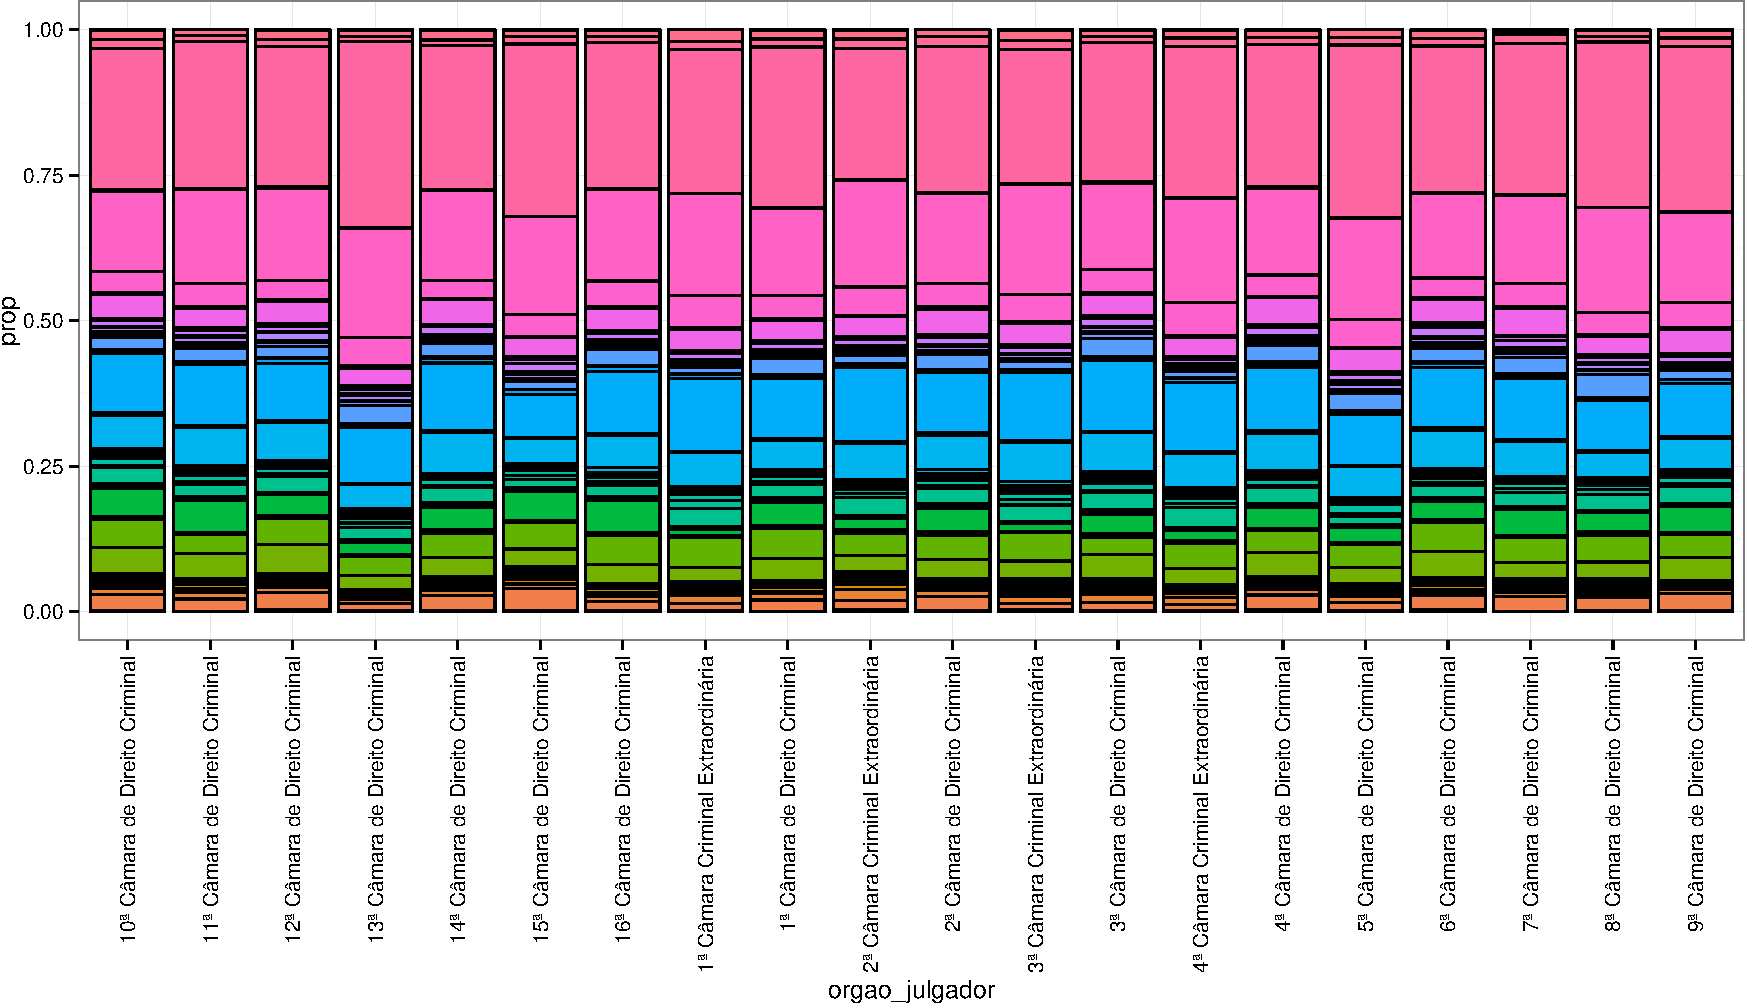
\includegraphics{/tmp/RtmpWS90dg/preview-ef06ab1be1f.dir/eped_files/figure-latex/unnamed-chunk-9-1.pdf}
\caption{Distribuição dos assuntos em cada câmara.}
\end{figure}

Buscando homogeneizar os grupos, definimos um algoritmo que cria uma
reamostragem de processos, dentro de cada câmara, a partir dos assuntos,
mas utilizando como base a proporção geral dos assuntos na base de
dados. Dessa forma, foi possível construir uma base com o mesmo número
de observações, mas com a mesma distribuição de assuntos dentro de cada
câmara. Observe, na Figura XXX, como as câmaras ficaram próximas.

\begin{figure}[htbp]
\centering
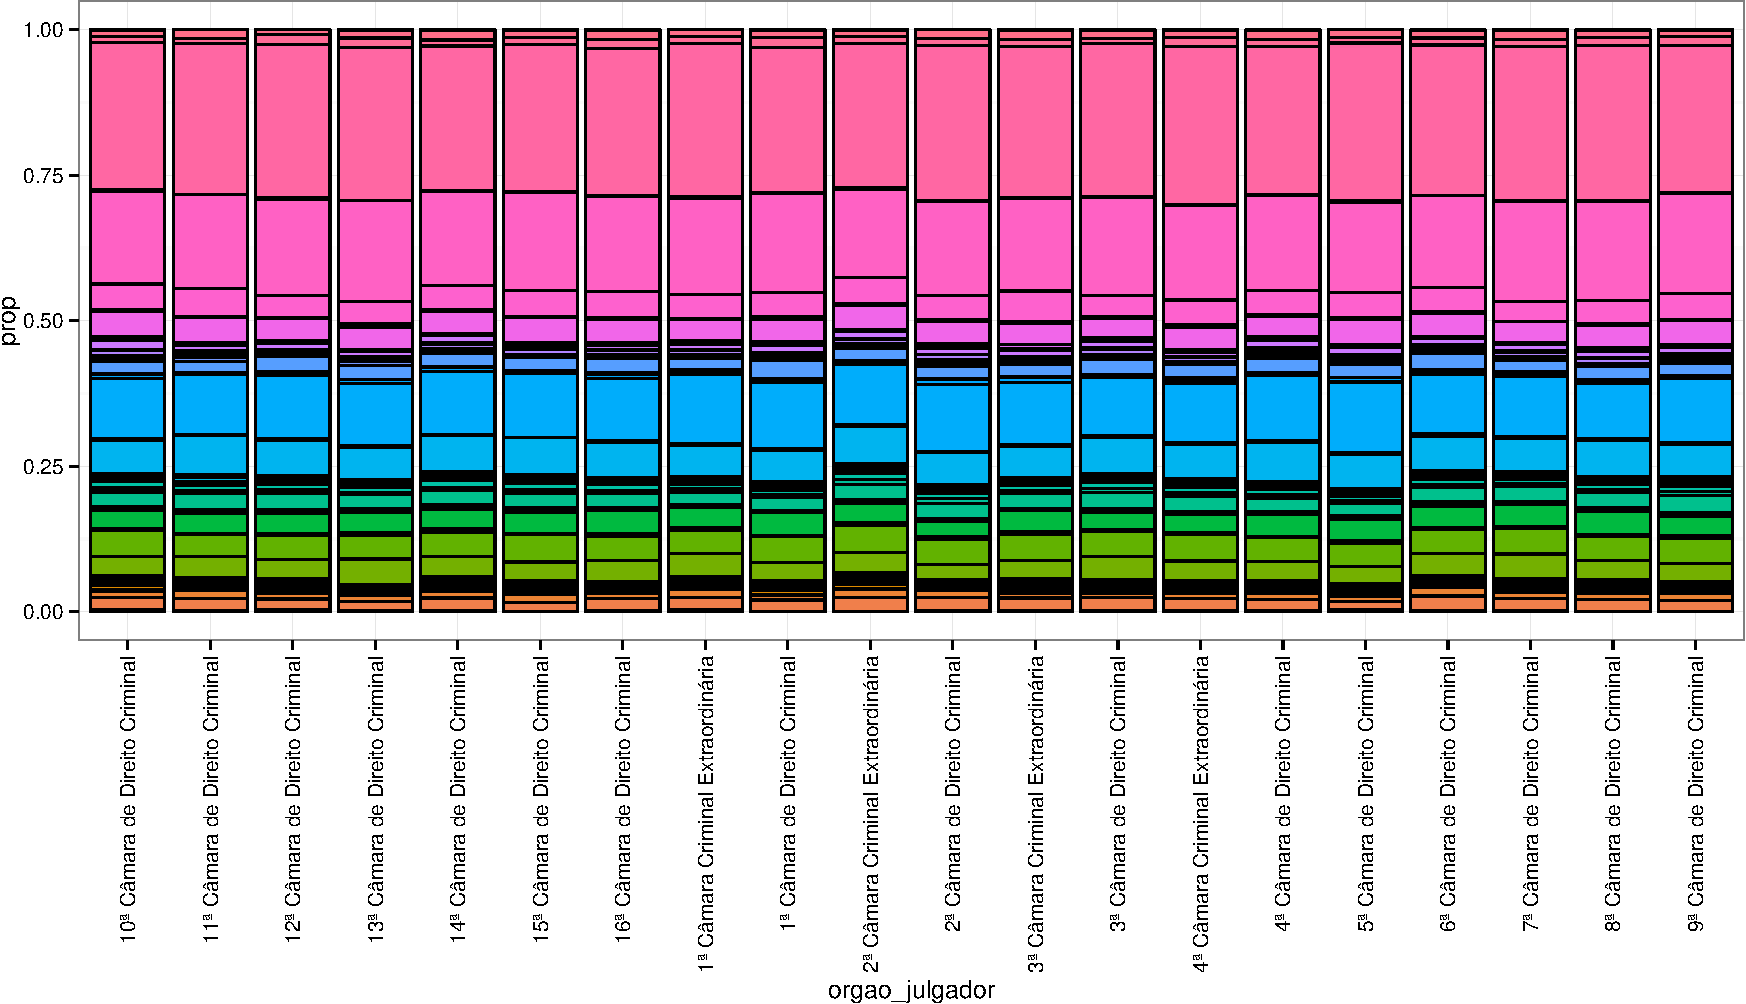
\includegraphics{/tmp/RtmpWS90dg/preview-ef06ab1be1f.dir/eped_files/figure-latex/unnamed-chunk-10-1.pdf}
\caption{Distribuição dos assuntos em cada câmara, base homogeneizada.}
\end{figure}

A Tabela XXX mostra os resultados para a base de dados homogeneizada.
Podemos observar que, mesmo realizando esse ajuste, os resultados das
câmaras permanecem distintos.

\begin{longtable}[c]{@{}rrrrrr@{}}
\caption{Tabela de frequências dos resultados dos processos segundo
órgao julgador, a partir de base homogeneizada.}\tabularnewline
\toprule
Órgão julgador & negaram & outros & parcialmente & provido &
total\tabularnewline
\midrule
\endfirsthead
\toprule
Órgão julgador & negaram & outros & parcialmente & provido &
total\tabularnewline
\midrule
\endhead
4ª Câmara de Direito Criminal & 3070 (80.7\%) & 18 (0.5\%) & 518
(13.6\%) & 197 (5.2\%) & 3803 (100\%)\tabularnewline
3ª Câmara de Direito Criminal & 2369 (67.1\%) & 24 (0.7\%) & 820
(23.2\%) & 318 (9.0\%) & 3531 (100\%)\tabularnewline
14ª Câmara de Direito Criminal & 1816 (52.7\%) & 18 (0.5\%) & 1152
(33.4\%) & 458 (13.3\%) & 3444 (100\%)\tabularnewline
3ª Câmara Criminal Extraordinária & 2416 (71.3\%) & 14 (0.4\%) & 426
(12.6\%) & 533 (15.7\%) & 3389 (100\%)\tabularnewline
4ª Câmara Criminal Extraordinária & 1501 (44.3\%) & 4 (0.1\%) & 1099
(32.5\%) & 781 (23.1\%) & 3385 (100\%)\tabularnewline
9ª Câmara de Direito Criminal & 2247 (69.5\%) & 10 (0.3\%) & 785
(24.3\%) & 192 (5.9\%) & 3234 (100\%)\tabularnewline
1ª Câmara Criminal Extraordinária & 1638 (51.0\%) & 16 (0.5\%) & 843
(26.3\%) & 712 (22.2\%) & 3209 (100\%)\tabularnewline
10ª Câmara de Direito Criminal & 1498 (47.2\%) & 19 (0.6\%) & 1320
(41.6\%) & 338 (10.6\%) & 3175 (100\%)\tabularnewline
2ª Câmara Criminal Extraordinária & 1830 (57.6\%) & 12 (0.4\%) & 752
(23.7\%) & 581 (18.3\%) & 3175 (100\%)\tabularnewline
7ª Câmara de Direito Criminal & 1787 (56.9\%) & 16 (0.5\%) & 919
(29.3\%) & 417 (13.3\%) & 3139 (100\%)\tabularnewline
8ª Câmara de Direito Criminal & 1626 (54.2\%) & 15 (0.5\%) & 737
(24.6\%) & 624 (20.8\%) & 3002 (100\%)\tabularnewline
16ª Câmara de Direito Criminal & 976 (35.2\%) & 26 (0.9\%) & 1300
(46.9\%) & 472 (17.0\%) & 2774 (100\%)\tabularnewline
11ª Câmara de Direito Criminal & 1218 (44.1\%) & 14 (0.5\%) & 1184
(42.9\%) & 346 (12.5\%) & 2762 (100\%)\tabularnewline
12ª Câmara de Direito Criminal & 404 (15.6\%) & 40 (1.5\%) & 1379
(53.2\%) & 767 (29.6\%) & 2590 (100\%)\tabularnewline
6ª Câmara de Direito Criminal & 1985 (77.9\%) & 26 (1.0\%) & 376
(14.8\%) & 160 (6.3\%) & 2547 (100\%)\tabularnewline
13ª Câmara de Direito Criminal & 1301 (52.9\%) & 20 (0.8\%) & 930
(37.8\%) & 208 (8.5\%) & 2459 (100\%)\tabularnewline
2ª Câmara de Direito Criminal & 527 (22.9\%) & 2 (0.1\%) & 1271 (55.1\%)
& 506 (21.9\%) & 2306 (100\%)\tabularnewline
1ª Câmara de Direito Criminal & 571 (25.7\%) & 6 (0.3\%) & 1240 (55.9\%)
& 401 (18.1\%) & 2218 (100\%)\tabularnewline
5ª Câmara de Direito Criminal & 1251 (70.8\%) & 9 (0.5\%) & 372 (21.0\%)
& 136 (7.7\%) & 1768 (100\%)\tabularnewline
total & 30777 (53.4\%) & 315 (0.547\%) & 18143 (31.5\%) & 8390 (14.6\%)
& 57625 (100\%)\tabularnewline
\bottomrule
\end{longtable}

\subsubsection{Relator}\label{relator}

A análise por órgão julgador nos dá a intuição de que pode ser que os
resultados dos processos sejam efeito de diferentes formas que os
magistrados têm ao conduzir os processos.

A Tabela XXX mostra a distribuição dos resultados dos processos em
relação aos quinze relatores com maior volume de processos. Na
comparação, é possível notar que existem discrepâncias significativas na
proporção de resultados desfavoráveis, chegando a ser maior do que 85\%
em dois casos. Seria interessante investigar esses casos mais a fundo,
pois a diferença observada poderia ser explicada tanto por uma diferença
na interpretação quanto por diferenças dos perfis dos processos de cada
relator.

\begin{longtable}[c]{@{}rrrrrr@{}}
\caption{Tabela de frequências dos resultados dos processos segundo
relator.}\tabularnewline
\toprule
Relator & negaram & outros & parcialmente & provido &
total\tabularnewline
\midrule
\endfirsthead
\toprule
Relator & negaram & outros & parcialmente & provido &
total\tabularnewline
\midrule
\endhead
Eduardo Abdalla & 599 (50.3\%) & 6 (0.5\%) & 369 (31.0\%) & 218 (18.3\%)
& 1192 (100\%)\tabularnewline
Aguinaldo de Freitas Filho & 804 (68.2\%) & 2 (0.2\%) & 189 (16.0\%) &
184 (15.6\%) & 1179 (100\%)\tabularnewline
Cesar Augusto Andrade de Castro & 610 (53.1\%) & 2 (0.2\%) & 322
(28.0\%) & 214 (18.6\%) & 1148 (100\%)\tabularnewline
Alexandre Almeida & 454 (40.1\%) & 1 (0.1\%) & 385 (34.0\%) & 293
(25.9\%) & 1133 (100\%)\tabularnewline
Julio Caio Farto Salles & 747 (66.1\%) & 1 (0.1\%) & 193 (17.1\%) & 189
(16.7\%) & 1130 (100\%)\tabularnewline
Luis Augusto de Sampaio Arruda & 565 (50.0\%) & 6 (0.5\%) & 388 (34.4\%)
& 170 (15.1\%) & 1129 (100\%)\tabularnewline
Mauricio Valala & 502 (47.2\%) & 6 (0.6\%) & 341 (32.1\%) & 214 (20.1\%)
& 1063 (100\%)\tabularnewline
Edison Brandão & 931 (87.7\%) & 9 (0.8\%) & 100 (9.4\%) & 22 (2.1\%) &
1062 (100\%)\tabularnewline
Ivana David & 883 (86.5\%) & 6 (0.6\%) & 71 (7.0\%) & 61 (6.0\%) & 1021
(100\%)\tabularnewline
Zorzi Rocha & 852 (84.4\%) & 1 (0.1\%) & 98 (9.7\%) & 59 (5.8\%) & 1010
(100\%)\tabularnewline
Luiz Antonio Cardoso & 509 (51.1\%) & 9 (0.9\%) & 375 (37.6\%) & 104
(10.4\%) & 997 (100\%)\tabularnewline
Roberto Mortari & 601 (63.5\%) & 5 (0.5\%) & 232 (24.5\%) & 109 (11.5\%)
& 947 (100\%)\tabularnewline
Ruy Alberto Leme Cavalheiro & 672 (72.0\%) & 5 (0.5\%) & 118 (12.6\%) &
138 (14.8\%) & 933 (100\%)\tabularnewline
Lauro Mens de Mello & 536 (57.9\%) & 4 (0.4\%) & 250 (27.0\%) & 135
(14.6\%) & 925 (100\%)\tabularnewline
total & 31059 (53.9\%) & 347 (0.638\%) & 17877 (31\%) & 8342 (14.5\%) &
57625 (100\%)\tabularnewline
\bottomrule
\end{longtable}

Buscando verificar se existe viés por conta dos assuntos dos processos,
aplicamos a mesma análise realizada nas câmaras afim de homogeneizar os
relatores. Assim como no caso das câmaras, as discrepâncias foram
mantidas.

\subsubsection{Data de julgamento}\label{data-de-julgamento}

A Figura XXX mostra as proporções de resultados dos processos em cada
mês. É possível notar que entre os meses de junho e setembro houve um
aumento significativo na proporção de recursos negados, caindo novamente
entre setembro e dezembro.

\begin{figure}[htbp]
\centering
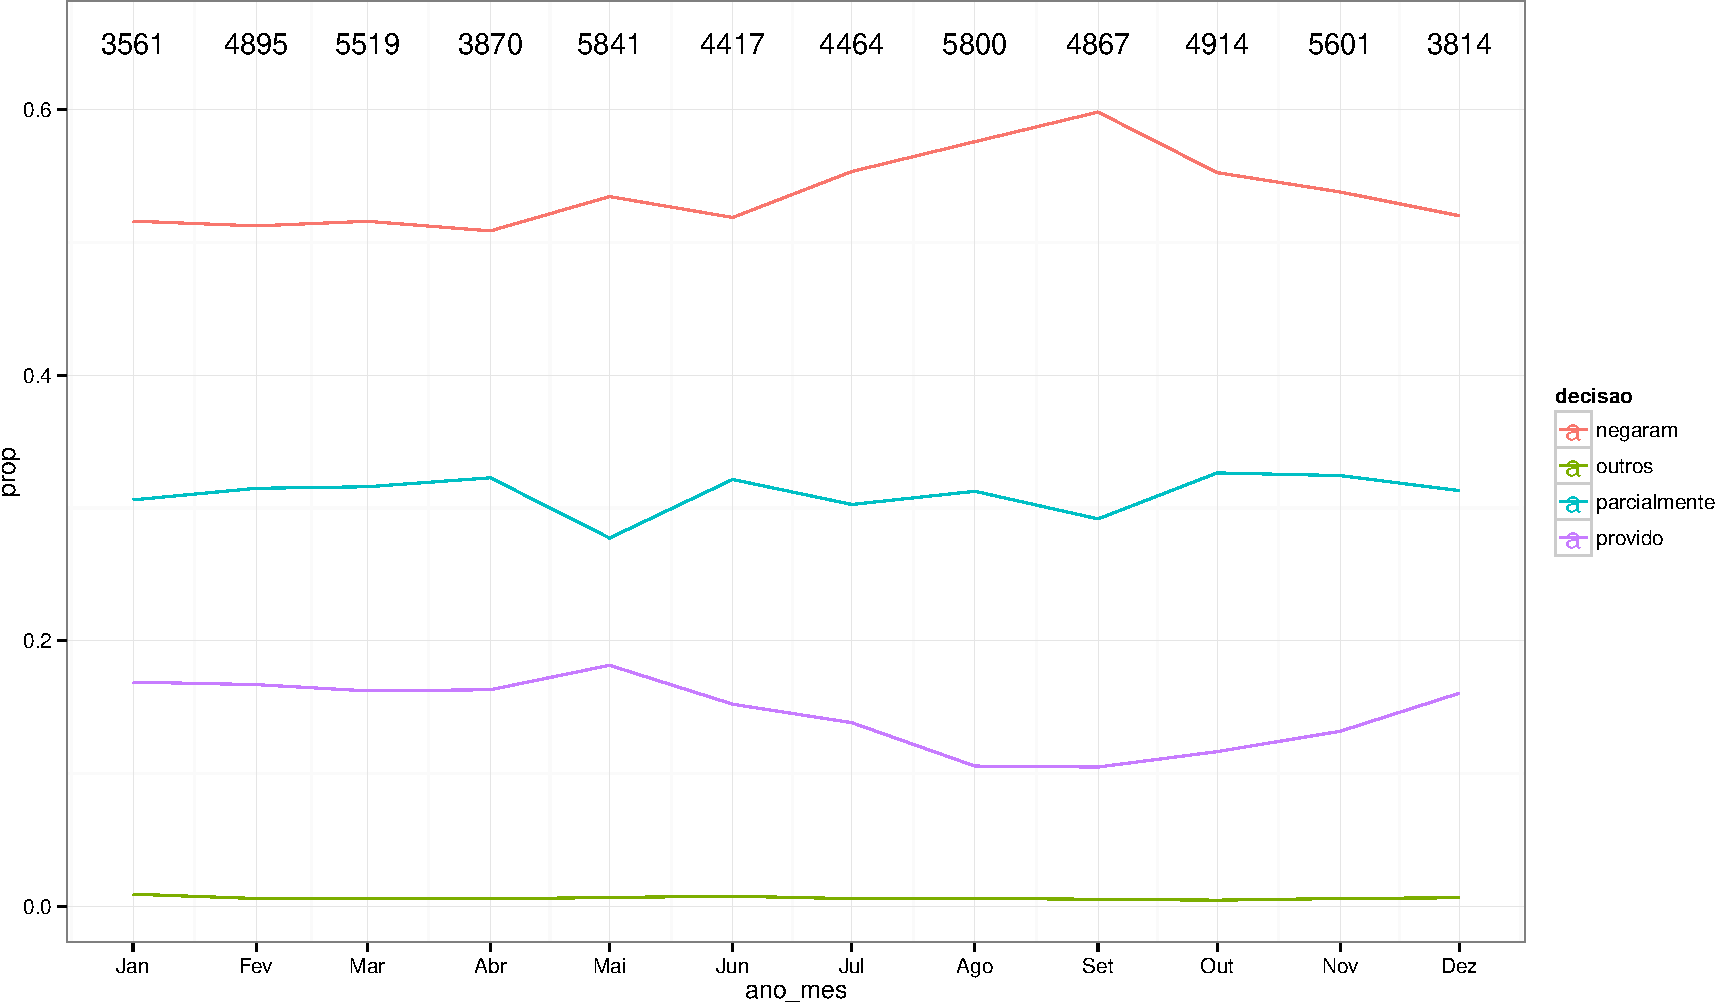
\includegraphics{/tmp/RtmpWS90dg/preview-ef06ab1be1f.dir/eped_files/figure-latex/unnamed-chunk-13-1.pdf}
\caption{Proporções resultados dos processos por mês.}
\end{figure}

\subsection{Discussão}\label{discussao}

XXX

\subsection{Considerações finais}\label{consideracoes-finais}

XXX

\end{document}
